\chapter{Predicción de resultados}

\section{Introducción}
Lo que se pretende hacer en este capítulo es plantear modelos que nos permitan predecir cómo quedará el ranking al final de la jornada que aún no ha comenzado, para lo que hay que estimar las distintas probabilidades de que gane un equipo, el rival o empaten para cada partido que se va a disputar. Los modelos para predecir los resultados finales del partido pueden ser de lo más variado y estar basados en todo tipo de criterios.\\

En \cite{refpred1} podemos encontrar dos modelos que se aplican para predecir los resultados de la liga alemana en las temporadas 1999/2000, 2000/2001 y 2001/2002:
\begin{itemize}
	\item Uno basado en los \textbf{mercados de predicción} en el que los precios de mercado nos ofrecen una visión agregada de la información pública y privada de la que disponen todos los participantes. El funcionamiento de los mercados de predicción se explica en \cite[Tabla II]{refpred1} y el modelo de cálculo de probabilidades se plantea en \cite[pág 62]{refpred1}.
	\item El otro modelo está basado en las \textbf{apuestas}. En él podemos realizar el cálculo de las probabilidades como se plantea en \cite[págs 62-63]{refpred1}, basándonos en las predicciones que realizan los corredores de apuestas para imponer los precios.
\end{itemize}

Son dos métodos de predicción relativamente aceptables teniendo mayor exactitud que otros métodos como el de \textit{selección aleatoria} y el de \textit{victoria del equipo local} con los que se comparan en \cite[págs 64-66]{refpred1}, aunque la tasa de acierto entre los dos modelos propuestos, el de los mercados de predicción y el de las apuestas, son muy similares.\\
Se puede aumentar la exactitud de las predicciones combinando ambos métodos, mediante ponderaciones del 50:50 o aplicando distintas reglas como \textit{solo predecir cuando las previsiones de ambos métodos coincidan} \cite[págs 66-67]{refpred1}.\\

En \cite{refpred2} se aplica el uso de \textbf{redes neuronales} para la predicción. En \cite[Section 2.1.]{refpred2} se explica el diseño de la red BP\footnote{Back-Propagation.}. Cada equipo tendrá tres tipos de redes BP que se corresponden con su fuerza y el problema de clasificación consiste en contrastar las fuerzas de los dos equipos: si A es más fuerte que B, es concordante o es más débil \cite[Section 2.2.]{refpred2}. Todos los partidos jugados serán los datos usados para el entrenamiento \cite[Section 3.1.]{refpred2} y la capa de salida consta de tres neuronas que se corresponden con la probabilidad de ganar, empatar y perder \cite[Section 3.2.]{refpred2} de forma que se pueda predecir el resultado del enfrentamiento como se muestra en \cite[Section 3.4.]{refpred2}.\\

En \cite{refpred3} se aplica un modelo autorregresivo integrado de media móvil o ARIMA que se usa en \textbf{series temporales} y que se basa en un conjunto de observaciones que se generan de forma secuencial. En \cite[Section E]{refpred3} se realiza la formulación matemática del modelo y en \cite[Section F]{refpred3} se muestran los resultados y el análisis de aplicarlo a tres equipos (uno de la zona alta, otro de la zona media y otro de la zona baja de la clasificación) de la liga india de críquet en el que se intenta predecir el resultado de los últimos 10 partidos de la temporada.\\

\section{Modelo propuesto}
En la sección anterior hemos visto algunos de los modelos que han sido propuestos para predecir los resultados de un partido que está por disputarse siguiendo distintos criterios. Ahora vamos a plantear uno propio que podamos aplicar a la Liga española de fútbol.\\

Para hacer una predicción tenemos que calcular tres probabilidades:
\begin{itemize}
	\item La probabilidad de que $a$ gane a $b$, que denotaremos como $P(a-b=1)$.
	\item La probabilidad de que $a$ y $b$ empaten, que denotaremos como $P(a-b=X)$.
	\item La probabilidad de que $a$ pierda ante $b$, que denotaremos como $P(a-b=2)$.
\end{itemize}
Y para estimarlas, proponemos tener en cuenta:
\begin{itemize}
	\item La posición relativa en la tabla, de donde obtendremos $P_{r}(a-b=1)$, $P_{r}(a-b=X)$ y $P_{r}(a-b=2)$.
	\item La tendencia de cada equipo a lo largo de los últimos partidos, de donde obtendremos $P_{s}(a-b=1)$, $P_{s}(a-b=X)$ y $P_{s}(a-b=2)$.
\end{itemize}

\subsection{Probabilidad basada en la posición relativa}
El valor va a depender de $r(a)-r(b)$, que pertenece al intervalo $[-(n-1),(n-1)] \backslash \{0\}$ donde $n$ es el número de equipos que hay en el ranking\footnote{Recordemos que $r(e)$ denota la posición que ocupa el elemento $e$ en el ranking $r$.}. En nuestro caso, aplicado a la Liga española de fútbol, dado que participan un total de 20 equipos el intervalo en cuestión es $[-19,19]$.\\

La idea es desarrollar un modelo lineal a trozos y optimizar sus parámetros usando un histórico de resultados.\\

\newpage

Lo primero es re-escalar el intervalo $[-19,19]$ en el $[0,1]$ mediante alguna función como por ejemplo
\begin{center}
	$ \psi: [-19,19] \longrightarrow [0,1]$\\
	$ t \longmapsto \dfrac{t+19}{38}$ \ .
\end{center}

Ahora debemos definir unos umbrales de victoria para el equipo local, empate y victoria visitante en tres escenarios muy distintos: \textit{el primero contra el último}, \textit{equipos en posiciones consecutivas} y \textit{el último contra el primero}. Gráficamente podemos resumirlo como se muestra en la figura \ref{fig:umbrales}.

\begin{figure}[htb]
		\centering
		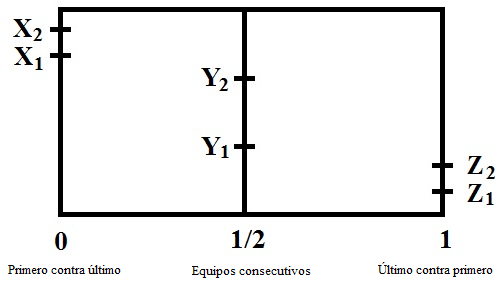
\includegraphics[scale=0.7]{images/umbrales.png}
		\caption{Gráfico de umbrales de victoria local, empate y victoria visitante.} \label{fig:umbrales}
\end{figure}

donde los valores $X_{1},X_{2},Y_{1},Y_{2},Z_{1},Z_{2} \in [0,1]$ se identifican del siguiente modo:
\begin{itemize}
	\item Si $a$ es el primero de la clasificación y $b$ el último:\\
	 	 
	 $\begin{cases}
	 	P_{r}(a-b=1)=X_{1}\\
	 	P_{r}(a-b=X)=X_{2}-X_{1} \ \ \ \ \ \ \ \text{siendo} \ 0 \leq X_{1} \leq X_{2} \leq 1.\\
	 	P_{r}(a-b=2)=1-X_{2} 
	 \end{cases}$\\
	 
	\item Análogamente, si $a$ y $b$ tienen puestos consecutivos en el ranking:\\
	
	$\begin{cases}
	P_{r}(a-b=1)=Y_{1}\\
	P_{r}(a-b=X)=Y_{2}-Y_{1} \ \ \ \ \ \ \ \text{siendo} \ 0 \leq Y_{1} \leq Y_{2} \leq 1.\\
	P_{r}(a-b=2)=1-Y_{2} 
	\end{cases}$\\
	
	\item Finalmente, si $a$ es el último de la clasificación y $b$ el primero:\\
	
	$\begin{cases}
	P_{r}(a-b=1)=Z_{1}\\
	P_{r}(a-b=X)=Z_{2}-Z_{1} \ \ \ \ \ \ \ \text{siendo} \ 0 \leq Z_{1} \leq Z_{2} \leq 1.\\
	P_{r}(a-b=2)=1-Z_{2} 
	\end{cases}$
\end{itemize}

Para el resto de escenarios tenemos que interpolar de forma lineal hallando 4 rectas (las que unen $X_{1}$ a $Y_{1}$, $Y_{1}$ a $Z_{1}$, $X_{2}$ a $Y_{2}$ y $Y_{2}$ a $Z_{2}$) tal y como se muestra en la figura \ref{fig:interpolar}.

\begin{figure}[htb]
	\centering
	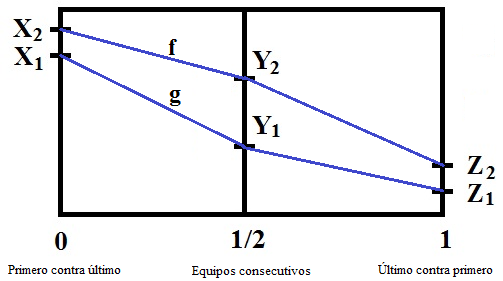
\includegraphics[scale=0.7]{images/interpolar.png}
	\caption{Gráfica de las funciones resultantes tras realizar la interpolación.} \label{fig:interpolar}
\end{figure}

De esta forma tenemos dos funciones $f,g:[0,1] \longrightarrow [0,1]$ tal que\\
$f(0)= X_{2}$ \ \ \ \ \ $f(1/2)= Y_{2}$ \ \ \ \ \ $f(1)= Z_{2}$ \ \ \ \ \ $f$ recta en $[0,1/2]$ y $[1/2,1]$\\
$g(0)= X_{1}$ \ \ \ \ \ $g(1/2)= Y_{1}$ \ \ \ \ \ $g(1)= Z_{1}$ \ \ \ \ \ $g$ recta en $[0,1/2]$ y $[1/2,1]$\\

De esta forma la predicción queda\\

$\begin{cases}
	P_{r}(a-b=1)=g(\psi (r(a)-r(b)))\\
	P_{r}(a-b=X)=f(\psi (r(a)-r(b)))-g(\psi (r(a)-r(b)))\\
	P_{r}(a-b=2)=1-f(\psi (r(a)-r(b)))
\end{cases}$
\ \\
\ \\
Para estimar los valores de $X_{1},X_{2},Y_{1},Y_{2},Z_{1},Z_{2}$ hay que optimizarlos teniendo en cuenta las siguientes restricciones:
\begin{itemize}
	\item $X_{1},X_{2},Y_{1},Y_{2},Z_{1},Z_{2} \in [0,1]$.
	\item $X_{1} \leq X_{2}$, $Y_{1} \leq Y_{2}$, $Z_{1} \leq Z_{2}$.
	\item $X_{1} \geq Y_{1} \geq Z_{1}$ y $X_{2} \geq Y_{2} \geq Z_{2}$.
\end{itemize}

\subsection{Probabilidad basada en la serie histórica de cada equipo}
Para cada equipo trabajaremos con dos series históricas: una serie con los resultados en casa y otra serie con los resultados fuera de casa, ambos ponderados según una función memoria. La idea de incorporar una función memoria es que el resultado de hace 9 partidos no tenga la misma importancia que puede tener el resultado del último.\\

\newpage

Para cada equipo $a$ trabajaremos con secuencias de resultados del tipo:
\begin{itemize}
\item Últimos 9 partidos como equipo local:
\begin{center}
	\begin{tabular}{|c|c|c|c|c|c|c|c|c|}
		\hline  t=1 & t=2 & t=3 & t=4 & t=5 & t=6 & t=7 & t=8 & t=9 \\ 
		\hline  1 & 1 & X & 1 & 2 & X & 1 & 1 & 1 \\
		\hline
	\end{tabular} 
\end{center}
donde $t=1$ es el partido (que se disputó como local) más antiguo que vamos a considerar y $t=9$ el último partido que se disputó (como local).
\item Últimos 9 partidos como equipo visitante:
\begin{center}
	\begin{tabular}{|c|c|c|c|c|c|c|c|c|}
		\hline  t=1 & t=2 & t=3 & t=4 & t=5 & t=6 & t=7 & t=8 & t=9 \\ 
		\hline  2 & 2 & X & 2 & 1 & X & 2 & X & 2 \\ 
		\hline
	\end{tabular} 
\end{center}
donde $t=1$ es el partido (disputado como visitante) más antiguo que vamos a considerar y $t=9$ el último partido que se disputó (como visitante).
\end{itemize}

De forma que para la jornada siguiente (la t=10) la probabilidad de que el equipo en cuestión gane, empate o pierda como local es:
\begin{center}
	$P_{l}(a - \star=1)=\dfrac{m(1)+m(2)+m(4)+m(7)+m(8)+m(9)}{\sum_{t=1}^{9}m(t)}$\\
	$P_{l}(a - \star=X)=\dfrac{m(3)+m(6)}{\sum_{t=1}^{9}m(t)}$ \ \ \ \
	$P_{l}(a - \star=2)=\dfrac{m(5)}{\sum_{t=1}^{9}m(t)}$
\end{center}
donde $m(t)$ es una función memoria típicamente creciente, lo que da mayor peso a los resultados de los últimos partidos, como la que se muestra en la figura \ref{fig:memoria}.

\begin{figure}[htb]
	\centering
	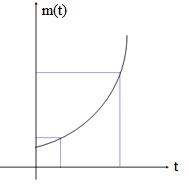
\includegraphics{images/memoria.jpg}
	\caption{Gráfica de la función memoria.} \label{fig:memoria}
\end{figure}
Análogamente se calculan las probabilidades para el siguiente partido como visitante:
\begin{center}
	$P_{v}(\star - a=1)=\dfrac{m(5)}{\sum_{t=1}^{9}m(t)}$ \ \ \ \
	$P_{v}(\star - a=X)=\dfrac{m(3)+m(6)+m(8)}{\sum_{t=1}^{9}m(t)}$\\
	$P_{v}(\star - a=2)=\dfrac{m(1)+m(2)+m(4)+m(7)+m(9)}{\sum_{t=1}^{9}m(t)}$
\end{center}
\ \\
Por tanto, para cada equipo tendremos las siguientes probabilidades:\\
$P_{l}(a - \star=1)$, $P_{l}(a - \star=X)$ y $P_{l}(a - \star=2)$ para los partidos como local y\\
$P_{v}(\star - a=1)$, $P_{v}(\star - a=X)$ y $P_{v}(\star - a=2)$ para los partidos como visitante.\\

Para pronosticar el resultado del enfrentamiento $a-b$ debemos conjuntar $P_{l}(a - \star)$ con $P_{v}(\star - b)$ usando la siguiente tabla:

\begin{center}
	\begin{tabular}{|c|c|c|c|}
	\hline  & $P_{l}(a - \star=1)$ & $P_{l}(a - \star=X)$ & $P_{l}(a - \star=2)$ \\ 
	\hline $P_{v}(\star - b=1)$ & $(1,0,0)$ & $(\frac{1}{2},\frac{1}{3},\frac{1}{6})$ & $(\frac{1}{4},\frac{1}{2},\frac{1}{4})$  \\ 
	\hline $P_{v}(\star - b=X)$ & $(\frac{1}{2},\frac{1}{3},\frac{1}{6})$ & $(0,1,0)$ & $(\frac{1}{6},\frac{1}{2},\frac{1}{3})$ \\ 
	\hline $P_{v}(\star - b=2)$ & $(\frac{1}{4},\frac{1}{2},\frac{1}{4})$ & $(\frac{1}{6},\frac{1}{2},\frac{1}{3})$ & $(0,0,1)$ \\ 
	\hline 
\end{tabular} 
\end{center}

En las tuplas de números de la tabla anterior, el primer número es el que usaremos para calcular $P_{s}(a-b=1)$, el segundo para $P_{s}(a-b=X)$ y el tercero para $P_{s}(a-b=2)$. Dicho número es por el que tenemos que multiplicar el producto de las entradas.\\

Por ejemplo, para calcular $P_{s}(a-b=1)$ la matriz que debemos usar es la compuesta por el primer elemento de cada tupla\\
\[
A_{1}= \left(\begin{array}{ccc}
1 & 1/2 & 1/4\\
1/2 & 0 & 1/6\\
1/4 & 1/6 & 0
\end{array} \right)
\]
de forma que
	\begin{center}
		$P_{s}(a-b=1)=$
	\end{center}
	$1\cdotp P_{l}(a - \star=1)P_{v}(\star - b=1) + \frac{1}{2}\cdotp P_{l}(a - \star=X)P_{v}(\star - b=1) + \frac{1}{4}\cdotp P_{l}(a - \star=2)P_{v}(\star - b=1)+$\\ 
	$\frac{1}{2}\cdotp P_{l}(a - \star=1)P_{v}(\star - b=X) + 0\cdotp P_{l}(a - \star=X)P_{v}(\star - b=X) + \frac{1}{6}\cdotp P_{l}(a - \star=2)P_{v}(\star - b=X)+$\\
	$\frac{1}{4}\cdotp P_{l}(a - \star=1)P_{v}(\star - b=2) + \frac{1}{6}\cdotp P_{l}(a - \star=X)P_{v}(\star - b=2) + 0\cdotp P_{l}(a - \star=2)P_{v}(\star - b=2)$. \\	

Aplicaremos un razonamiento análogo para calcular $P_{s}(a-b=X)$ y $P_{s}(a-b=2)$.

\subsection{Combinación}
Ahora contaremos con dos probabilidades: las probabilidades basadas en la posición relativa ($P_{r}(a-b=1) \ \ P_{r}(a-b=X) \ \ P_{r}(a-b=2)$) y las basadas en la serie histórica de cada equipo ($P_{s}(a-b=1) \ \ P_{s}(a-b=X) \ \ P_{s}(a-b=2)$).\\

Para conjugarlas usaremos una combinación convexa, tomamos $\lambda \in [0,1]$ y tenemos
\begin{center}
	$ P(a-b=1) = \lambda P_{r}(a-b=1) + (1-\lambda) P_{s}(a-b=1)$\\
	$ P(a-b=X) = \lambda P_{r}(a-b=X) + (1-\lambda) P_{s}(a-b=X)$\\
	$ P(a-b=2) = \lambda P_{r}(a-b=2) + (1-\lambda) P_{s}(a-b=2)$
\end{center}
debiendo optimizar $\lambda$ para obtener el mejor resultado posible entrenándolo sobre el histórico de datos.